\chapter{Bestimmung des Planck'schen Wirkungsquantums}
In diesem Versuch soll das Planck'sche Wirkungsquantum $\planck$ bestimmt werden. Diese Größe ist neben der Lichtgeschwindigkeit $\sol$ und der Gravitationskonstanten $\G$ die dritte fundamentale Naturkonstante der Physik. Sie beschreibt für schwingfähige Systeme das konstante Verhältnis aus der kleinstmöglichen Energieänderung und der Schwingungsfrequenz. Daraus folgt insbesondere, dass solche Systeme nur ganzzahlige Vielfache des sog. Schwingungsquants $\Delta E=\planck\nu$ aufnehmen können. Auch der Drehimpuls eines Systems kann sich nur um ganzzahlige Vielfache von $\hbar\equiv\frac{\planck}{2\pi}$ ändern. Dies sind jedoch nur einige der wichtigen Zusammenhänge, in denen die Planckkonstante eine wichtige Rolle spielt.

Die Bestimmung dieser fundamentalen Konstanten soll in diesem Versuch durch Messungen an Leuchtdioden, insbesondere der Feststellung von deren Wellenlängen über die Gleichung 
\begin{equation}
	E=\planck\nu
\end{equation}
bestimmt werden. Zwischen der Wellenlänge $\lambda$ und der Frequenz $\nu$ besteht dabei der bekannte Zusammenhang: $\sol=\lambda\nu$.

Da solche LEDs Halbleiter sind, muss in diesem Versuch auch eine gewisse Vertrautheit mit Grundlagen der Halbleiterphysik gegeben sein. Für diesen Versuch ist insbesondere das Resultat wichtig, dass die Wellenlänge des abgestrahlten Lichts nur von der sogenannten Gap-Energie $E_{\mathtt{gap}}$ abhängt, also von der Energie, die frei wird, wenn ein Elektron vom Leitungsband, der Energiezone, in der sich frei bewegliche und damit leitungsfähige Ladungsträger befinden, in das energetisch tieferliegende Valenzband übergeht. Diese Energie ist eine Materialkonstante, womit klar wird, dass die Farbe der LED nur von den verwendeten Halbleitern abhängt:
\begin{equation}
	\lambda=\frac{\planck\cdot\sol}{E_{\mathrm{gap}}}
\end{equation}
\section{Vorbereitung}
\begin{enumerate}
	\item Was versteht man unter Kohärenz? Was ist der Unterschied zwischen zeitlicher und räumlicher Kohärenz?
		\subitem Kohärenz: Hierunter versteht man, dass zwei Wellen ein gleiches bzw. ähnliches Verhalten in Bezug auf die Amplitudenänderung besitzen, das sich lediglich um eine feste Phasenbeziehung unterscheidet. In der Optik bezeichnet man zwei Wellen meist als kohärent, wenn deren Phasendifferenz konstant ist.
		\subitem Zeitliche Kohärenz: Als zeitliche Kohärenz bezeichnet man die Eigenschaft einer Welle, über ein gewisses Zeitintevall (die Kohärenzzeit $\tau_c$) in vorhersagbarer Art und Weise zu schwingen. Bei Lichtwellen beträgt die Kohärenzzeit typischerweiße $\tau_c=\SI{10}{\nano\second}$, was eine Frequenzunschärfe $\Delta\nu=\frac{1}{\tau_c}$ von ca. $\SI{100}{\mega\hertz}$ zur Folge hat. (Zum Vergleich: Sichtbares Licht hat eine Frequenz von ca. $430-770\,\si{\tera\hertz}$)
		\subitem Räumliche Kohärenz: Diese Eigenschaft ist speziell bei Experimenten wichtig, die die Interferenz zweier Wellen ausnutzen sollen, beispielsweiße beim Doppelspaltversuch. Hierbei werden zwei Punkte aus einer Welle herausgegriffen und zur Interferenz gebracht. Allerdings muss die Welle auf dem Gebiet, in dem die Punkte liegen, kohärent sein, damit dies möglich ist. Die maximale Größe dieses Gebiets entspricht dem Ausmaß der räumlichen Kohärenz.
	\item Leiten SIe anhand einer Skizze die Interferenzbedingung am Gitter $m\lambda=d\sin\theta$ her. 
		\subitem \begin{figure}[!hb]
			\centering
			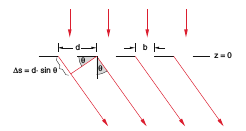
\includegraphics[]{interferenz}
			\caption{Interferenz am Gitter}
			\label{fig:Abb1}
		\end{figure}
		Wie in der Abbildung zu sehen, gilt für den Gangunterschied zweier Lichtstrahlen: $\Delta s=d\sin\theta$.
		Darüber hinaus müssen für konstruktive Interferenz die Strahlen die gleiche Phase aufweisen, also um ganzzahlige Vielfache der Wellenlänge versetzt sein: $\Delta s=m\lambda, m\in\mathbb{Z}$
		
		Insgesamt ergibt sich also:
		\begin{displaymath}
			\Delta s=m\lambda=d\sin\theta
		\end{displaymath}
	\pagebreak
	\item Wie sieht die Intensitätsverteilung eines Transmissionsgitters aus, das mit monochromatischem Licht beleuchtet wird?
		\subitem Die Intensitätsverteilung am Gitter wird beschrieben durch:
		\begin{displaymath}
			I(\theta)=I_S\cdot\frac{\sin^2[\pi(b/\lambda)\sin\theta]}{[\pi(b/\lambda)\sin\theta]^2}\cdot\frac{\sin^2[N\pi(d/\lambda)\sin\theta]}{\sin^2[\pi(d/\lambda)\sin\theta]}
		\end{displaymath}
		Hierbei handelt es sich um eine quadrierte sinc-Funktion als Envelope wie beim Einfachspalt, und eine vom jeweiligen Gitter abhängige Schwingung, die Nebenextrema produziert. Es ergibt sich folgende Intensitätsverteilung:
		\begin{figure}[!h]
			\centering
			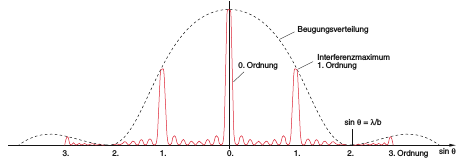
\includegraphics[]{intensitaet}
			\caption{Intensitätsverteilung am Beugungsgitter}
			\label{fig:Abb2}
		\end{figure}
	\item Skizzieren Sie den Verlauf der Dichten der Ladungsträger am p-n-Übergang, wenn eine äußere Spannung angelegt wurde.
		\subitem \begin{figure}[!h]
			\centering
			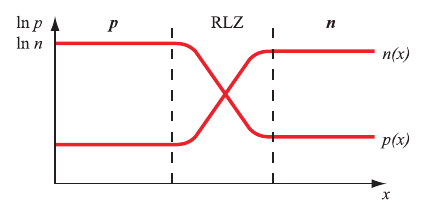
\includegraphics[]{pn}
			\caption{Ladungsträgerkonzentration bei Spannung in Durchlassrichtung}
			\label{fig:Abb3}
		\end{figure}
\end{enumerate}
\section{Durchführung}
\subsection{Farbfilter}
\begin{enumerate}
	\item Betrachten Sie die Säule mit den farbigen LEDs durch verschiedene Farbfilter. Bei der Verwendung des Rotfilters werden Sie feststellen, dass die rote LED heller zu sein scheint als der Rest. Das Rotfilter läßt das rote Licht also durch und blockiert die anderen Farben. Betrachten Sie die LEDs durch die anderen Filter: welche Farben werden „scharf“ durchgelassen, welche anderen Farbanteile transmittieren eventuell zusätzlich?
	\item Wie unterscheidet sich die pinke LED von den anderen einfarbigen LEDs?
	\item Erstellen Sie für das Grünfilter ein (subjektives) Intensitätsprofil. Tragen Sie auf der Abszisse die Farben auf (rot, orange, gelb, grün, blau, violett), auf der Ordinate die Intensität (in \%)
	\item Was verändert sich, wenn Sie zwei verschiedene Filter übereinander legen?
	\item Wie verändert sich bei den Filteraufgaben das Licht der weißen LED? Warum?
\end{enumerate}
\subsection{Bestimmung der Wellenlänge der LEDs}
\begin{enumerate}
	\item  Betrachten Sie die LED-Säule durch die Gitter. Neben der senkrechten Reihe von LEDs sehen Sie links und rechts davon virtuelle Bilder der LEDs. 
		\subitem a) Warum ist das virtuelle Bild nicht genauso punktförmig, wie das Urbild? Warum erscheint das virtuelle Bild ellipsenförmig mit einer "Verschmierung" der Farbe?
		\subitem b) Wie kann man erklären, dass der Abstand der virtuellen Bilder von der Mittelsenkrechten von der Farbe des Lichtes abhängt?
	\item Befestigen Sie das Din A3-Blatt an der Halterung (y-Richtung) und stellen Sie das Gitter in einem festen Abstand vor das LED-Array (x-Richtung). Bestimmen Sie mithilfe der Winkelfunktionen und der Vorbereitungsaufgaben die Wellenlänge der LEDs Hinweis: die LEDs weiß, pink, UV und IR können so nicht ausgemessen werden - warum nicht?
	\item Machen Sie eine Fehlerbetrachtung Ihrer Meßanordnung.
\end{enumerate}
\subsection{Bestimmung des Planck'schen Wirkungsquantums}
\begin{enumerate}
	\item Messen Sie die Vorwärtsspannungen der LEDs und tragen Sie sie gegen ihre Frequenz auf.
	\item Bestimmen Sie daraus das Planck'sche Wirkungsquantum.
	\item Bei diesen Messungen wurden große Fehler in Kauf genommen. Welche sind das, und wodurch werden sie verursacht?
	\item Benutzen Sie nun statt des Festspannungs-Steckernetzteils das regelbare Netzteil im Bereich von 0-5V. Erhöhen Sie die Spannung langsam, bis die LED gerade eben zu Leuchten beginnt. Die zugehörige Spannung ist die Spannung der LED. Wiederholen Sie die Messungen, indem Sie die Spannungen der LEDs gegen die Frequenz auftragen.
	\item Bestimmen Sie das Planck'sche Wirkungsquantum und diskutieren Sie die Fehler.
\end{enumerate}